\begin{frame}
  \begin{PointSix}{Learning Goals}
    \begin{itemize}
      \item \alert{Polarization.}
      \item \alert{Polarization in the subsurface.}
      \item \alert{Principles of an RC circuit.}
      \item \alert{Definition of chargeability.}
    \end{itemize}
  \end{PointSix}
\end{frame}

\begin{frame}
  \begin{PointSix}{Electric Polarization}
    What is electric polarization?
  \end{PointSix}
\end{frame}

\begin{frame}
  \begin{PointSix}{Electric Polarization}
    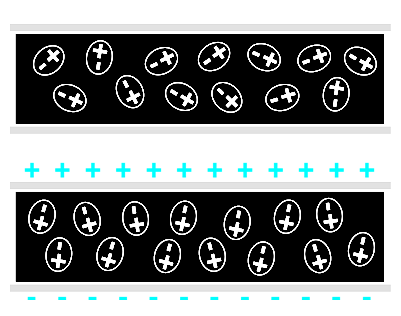
\includegraphics[width=1.0\textwidth]{Figures/InducedPolarization/diel.png}
  \end{PointSix}
\end{frame}

\begin{frame}
  \begin{PointSix}{Polarization (cf. magnetic susceptibility)}
  \small Electric polarization originates from effective charge separation in an (external) electric field. It opposes the external field an leads to an overall weakening of the total field.
    \begin{eqnarray}
      &\vec{P}& = \chi \varepsilon \vec{E} \\
      &\vec{D}& = \varepsilon \vec{E} + \vec{P}
    \end{eqnarray}
  \end{PointSix}
\end{frame}

\begin{frame}
  \begin{PointSix}{Polarization in sub-surface: Membrane Polarization}

    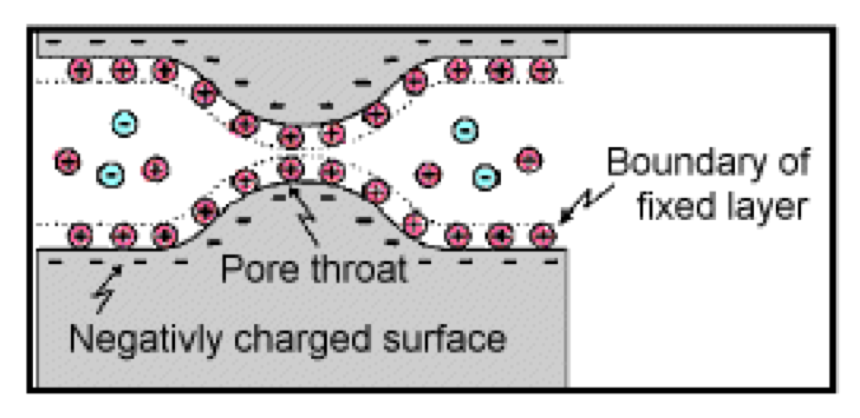
\includegraphics[width=0.5\linewidth]{Figures/InducedPolarization/MembranePotential1_GPG.png}
    \tiny [EOS, UBC 2022]
    \small
    \begin{itemize}
      \item Electric double layer forms in water-filled pore space.
    \end{itemize}  
  \end{PointSix}
\end{frame}

\begin{frame}
  \begin{PointSix}{Polarization in sub-surface: Membrane Polarization}

    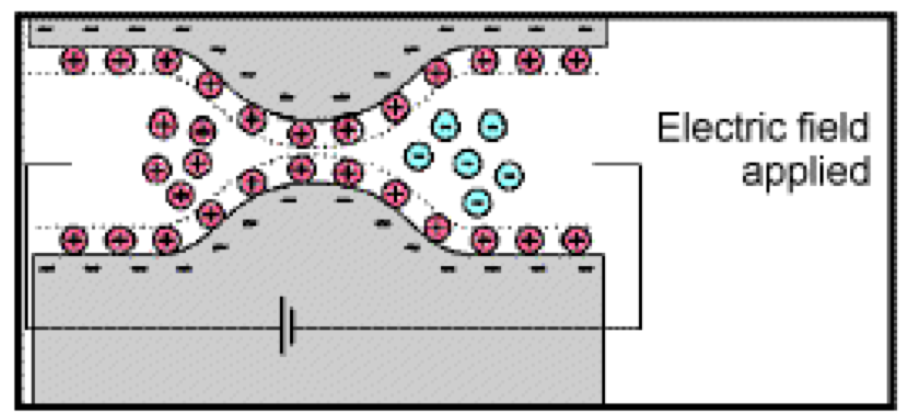
\includegraphics[width=0.5\linewidth]{Figures/InducedPolarization/MembranePotential2_EOS_UBC.png}
    \tiny [EOS, UBC 2022]

    \small
    \begin{itemize}
      \item Constrictions in pores leads to charge accumulation
    \end{itemize}  
  \end{PointSix}
\end{frame}

\begin{frame}
  \begin{PointSix}{Polarization in sub-surface: Membrane Polarization}

    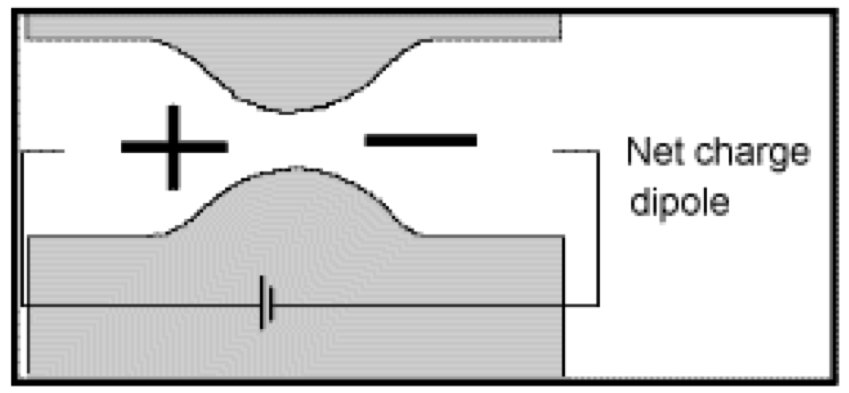
\includegraphics[width=0.5\linewidth]{Figures/InducedPolarization/MembranePotential3_EOS_UBC.png}
    \tiny [EOS, UBC 2022]

    \small
    \begin{itemize}
      \item Constrictions in pores leads to charge accumulation
      \item This can result in a macroscopic polarization
    \end{itemize}  
  \end{PointSix}
\end{frame}

\begin{frame}{Plants \& Roots}
  %  \begin{PointSix}{Polarization in Subsurface (Organic targets)}
      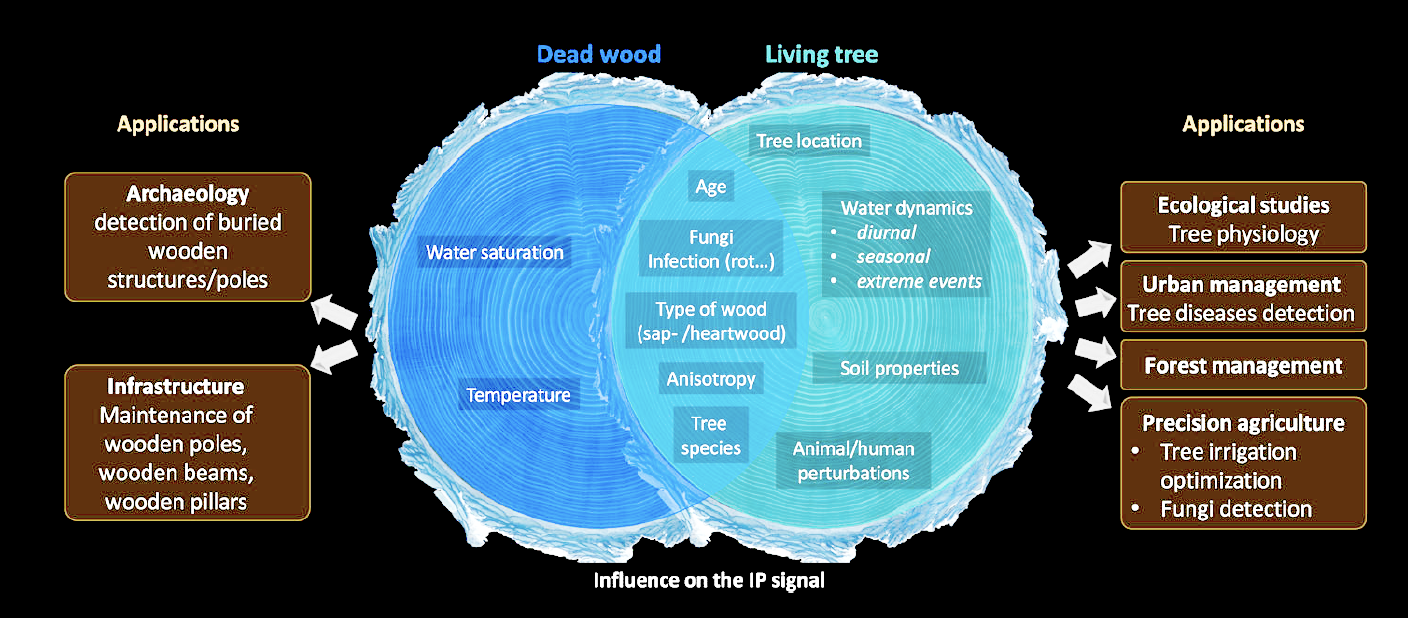
\includegraphics[width=1.0\textwidth]{Figures/InducedPolarization/IP_Tree_Kessouri2019_NearSurfaceGeophysics.png}
    
  
    \tiny [Kessouri et al., 2019, Near Surf. Geophys.]
  %  \end{PointSix}
  \end{frame}

  \begin{frame}{Plants \& Roots}
    %  \begin{PointSix}{Polarization in Subsurface (Organic targets)}
        
\includegraphics[width=0.5\textwidth]{Figures/InducedPolarization/IPRoots_2021.png}
        
\includegraphics[width=0.5\textwidth]{Figures/InducedPolarization/IPRoots2_2021.png}
      
    
   %   \tiny [Kessouri et al., 2019, Near Surf. Geophys.]
    %  \end{PointSix}
    \end{frame}

\begin{frame}{Microbial activity in soils}
%  \begin{PointSix}{Polarization in Subsurface (Microbes)}
    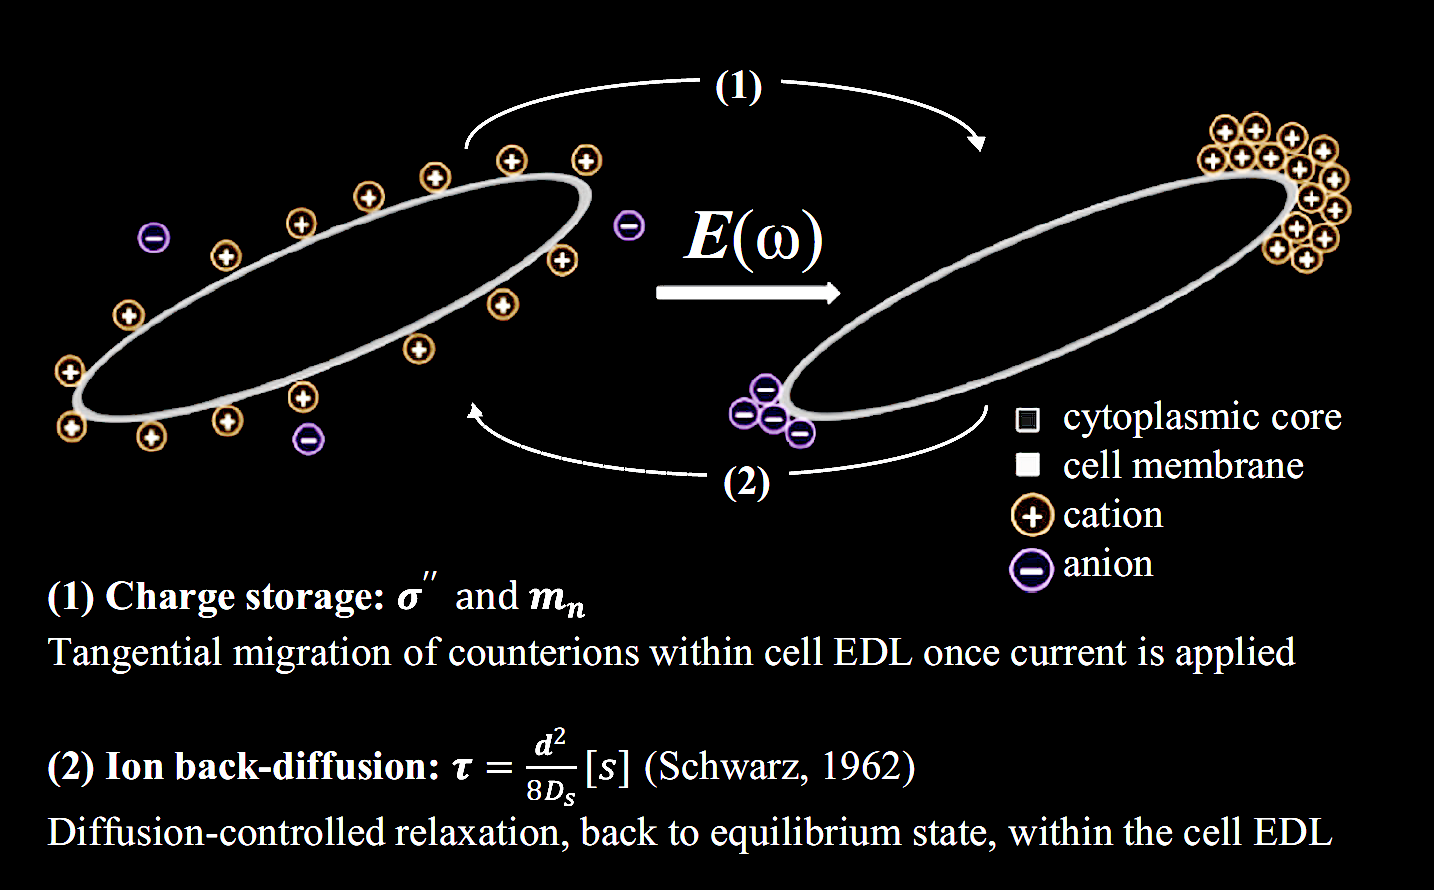
\includegraphics[width=0.6\textwidth]{Figures/InducedPolarization/IP_Microbes_Kessouri2019_NearSurfaceGeophysics.png}
  

  \tiny [Kessouri et al., 2019, Near Surf. Geophys.]
%  \end{PointSix}
\end{frame}

\begin{frame}
  \begin{PointSix}{Electric Polarization}
    How does polarization in the sub-surface appear within a resistivity setup?
  \end{PointSix}
\end{frame}

\begin{frame}
  \begin{PointSix}{Electric Polarization}
    How does polarization in the sub-surface appear within a resistivity setup?

    $\rightarrow$ This is equivalent to an RC-Circuit.
  \end{PointSix}
\end{frame}

\begin{frame}
  \begin{PointSix}{RC Circuits}
   % RESISTOR with battery and arrow

    \begin{tikzpicture}
      
      \newcommand\EMF{\mathcal{E}};
      \colorlet{Icol}{blue!50!black}
      \colorlet{Ccol}{orange!90!black}
      \colorlet{Rcol}{Karminrot}
      \colorlet{loopcol}{red!90!black!25}
      \colorlet{pluscol}{red!60!black}
      \colorlet{minuscol}{blue!60!black}
      \tikzstyle{EMF}=[battery1,l=$\EMF$];
      \tikzstyle{internal R}=[R,color=Rcol,Rcol,l=$r$,/tikz/circuitikz/bipoles/length=30pt];
      \tikzstyle{loop}=[->,red!90!black!25];
      \tikzstyle{loop label}=[loopcol,fill=white,scale=0.8,inner sep=1];
      \tikzstyle{thick R}=[R,color=Rcol,thick,Rcol,l=$R$];
      
      \begin{scope}[rotate=-90,transform shape]
        \fill[pattern = crosshatch dots,pattern color = brown!80!red] (0.5,-0.5) rectangle ++(6,9);
       % \node[rotate=90] at (0.25,1.5) {Surface};
        \draw (0,7)
        to (4,7) 
        to[C,color=Rcol,thick,l={{{{\rotatebox[origin=c]{90}{$C$}}}}}] (4,3) 
        to[R,color=Rcol,thick,l={{{{\rotatebox[origin=c]{90}{$R$}}}}}] (4,0)
        to (0,0) 
        to [ammeter, color=white] (0,7);
        \node[rotate=90,above] at (0,7) {$B$};
        \node[rotate=90,above] at (0,0) {$A$};
   
       % \node[rotate=90] at (0,4) {$\Delta V$};
          %  \draw[->,red] (0.5, 2.15) --++ (1.2,0) node[midway,above=1] {current $I$};
          %  \draw[->,red] (0.5,-0.15) --++ (1.2,0) node[midway,below=1] {electron flow};
        \end{scope}
        \draw[-,color=white] (2,-0.8) -- (2,1.2);
        \draw[-,color=white] (2,1.2) -- node[above] {$\Delta$ U} (5,1.2);
        \draw[-,color=white] (5,1.2) -- (5,-0.8);
        
        \node[above] at (2,1.2) {$M$};
        \node[above] at (5,1.2) {$N$};
    \end{tikzpicture}
  \end{PointSix}
\end{frame}

%https://openpress.usask.ca/physics155/chapter/6-5-rc-circuits/
%https://www.coursehero.com/study-guides/boundless-physics/rc-circuits/

\begin{frame}
  \begin{PointSix}{Electric Polarization}
   \small
   \begin{center}
    How does the current behave in an RC circuit connected to a DC battery? Start with Kirchoffs law that The  sum of the potential differences around any closed loop is zero.
   \end{center}
  \end{PointSix}
\end{frame}



\begin{frame}
  \begin{PointSix}{RC - Circuit: Charging}
  \begin{eqnarray*}
    V - V_R - V_C = 0 \\
   \end{eqnarray*}
   \small
    What is the voltage drop across a capacitor? 
  \end{PointSix}
\end{frame}

\begin{frame}
  \begin{PointSix}{Electric Polarization}
    \begin{eqnarray*}
      V_C = \frac{q}{C} \\
     \end{eqnarray*}
   \begin{center}
    \small
    It depends on the charge accumulation q(t) and the material constants (C) including the geometry.
   \end{center}
  \end{PointSix}
\end{frame}

\begin{frame}{RC - Circuit: Charging}
  \begin{eqnarray*}
    V - V_R - V_C = 0 \\
    V - RI - \frac{q}{C} = 0 \\
    V - R\frac{dq}{dt}-\frac{1}{C}q = 0  
  \end{eqnarray*}
  \small
  Can be solved with separation of Variables.

\end{frame}

\begin{frame}{RC - Circuit: Charging}
  \begin{eqnarray*}
    &\frac{dq}{dt} = \frac{UC - q}{RC} \\
    &\rightarrow \frac{1}{UC-q}dq = \frac{1}{RC} dt \\
    &\rightarrow q(t) = CV(1-e^{-\frac{t}{RC}}) \\
  \end{eqnarray*}

  \begin{equation}
    \alert{I(t) = \frac{dq(t)}{dt}=\frac{V}{R}e^{-\frac{t}{RC}}=I_0e^{-\frac{t}{RC}}} 
    %= \frac{dq(t)}{dt}=I_0e^{-\frac{t}{RC}}}
  \end{equation}


\end{frame}

\begin{frame}{RC - Circuit: Decharging}
  For decharging $V=0$ (battery disconnected):

  \begin{equation}
    \alert{I(t) = -\frac{Q}{RC}e^{-\frac{t}{RC}}} 
    %= \frac{dq(t)}{dt}=I_0e^{-\frac{t}{RC}}}
  \end{equation}

  (Exercises.)

\end{frame}


% \begin{frame}{Spectral Induced Polarization}
%   \begin{eqnarray}
%     V(t) = V_0e^{i\omega t} \\
%     U_c = \frac{q}{C} \rightarrow I(t)\\
%         = \frac{1}{C}\frac{dU}{dt} = \frac{j\omega}{C}U(t)
%   \end{eqnarray}
% \end{frame}

% \begin{frame}{Spectral Induced Polarization}
%   \begin{eqnarray}
%     V(t) = V_0e^{i\omega t} \\
%     U_c = \frac{q}{C} \rightarrow I(t)\\
%         = \frac{1}{C}\frac{dU}{dt} = \frac{j\omega}{C}U(t)
%   \end{eqnarray}
% \end{frame}

% \begin{frame}{Spectral Induced Polarization}
%   \begin{eqnarray}
%     V(t) = I(t)R + \frac{C}{j\omega}I(t) \\
%          = (R + \frac{C}{j\omega})I(t) \\
%          = (R - j\frac{C}{\omega})I(t)
%   \end{eqnarray}
% \end{frame}


\begin{frame}
  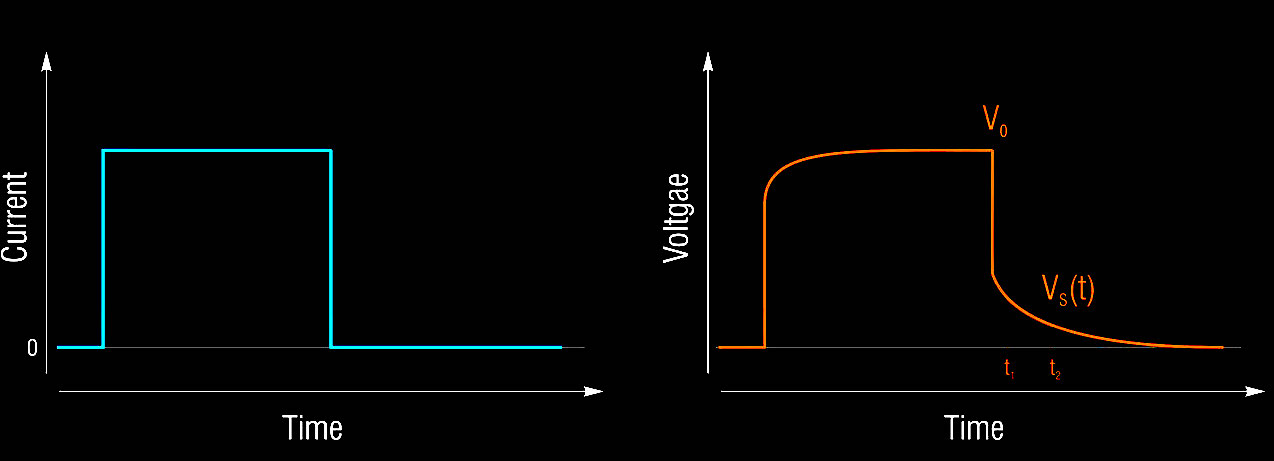
\includegraphics[width=1.0\linewidth]{Figures/InducedPolarization/IP-curve_EverestGeophysics.jpg}

  \tiny[Source: Everest Geophysics (Spain)]
\end{frame}


\begin{frame}
  \begin{PointSix}{Chargeability}
    \small
    The chargeability $M$ [ms] is the quantitiy measured in time-domain, induced polarization:
    $$
      M = \frac{1}{V_0}\int_{t_1}^{t_2}V(t)
    $$
  \end{PointSix}
\end{frame}


\begin{frame}{Examples}
  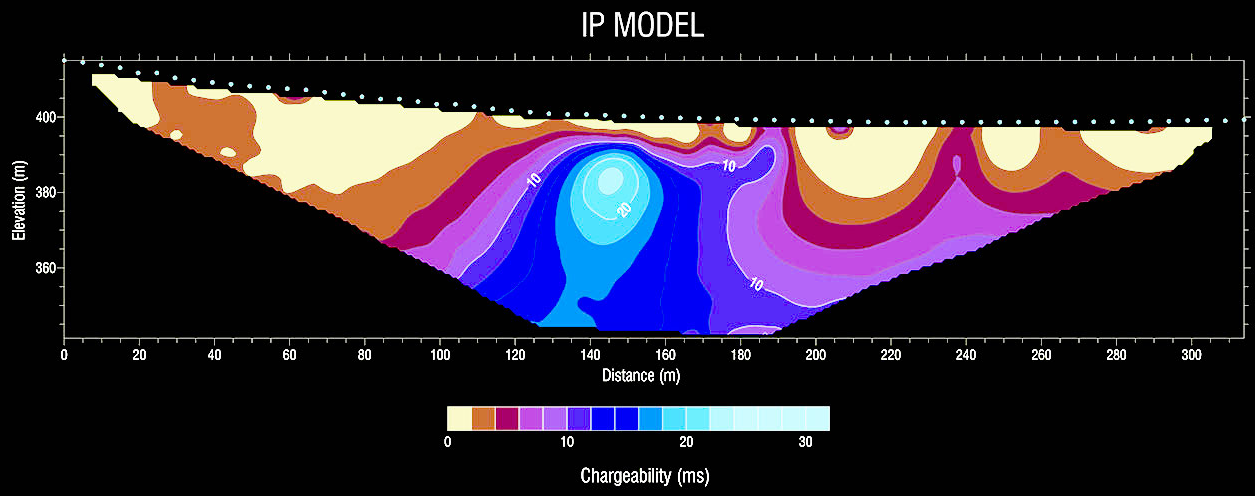
\includegraphics[width=0.8\linewidth]{Figures/InducedPolarization/resistivity-and-chargeability_ip_EverestGeophysics.png}

  \tiny[Source: Everest Geophysics (Spain)]
\end{frame}

\begin{frame}{Examples}
  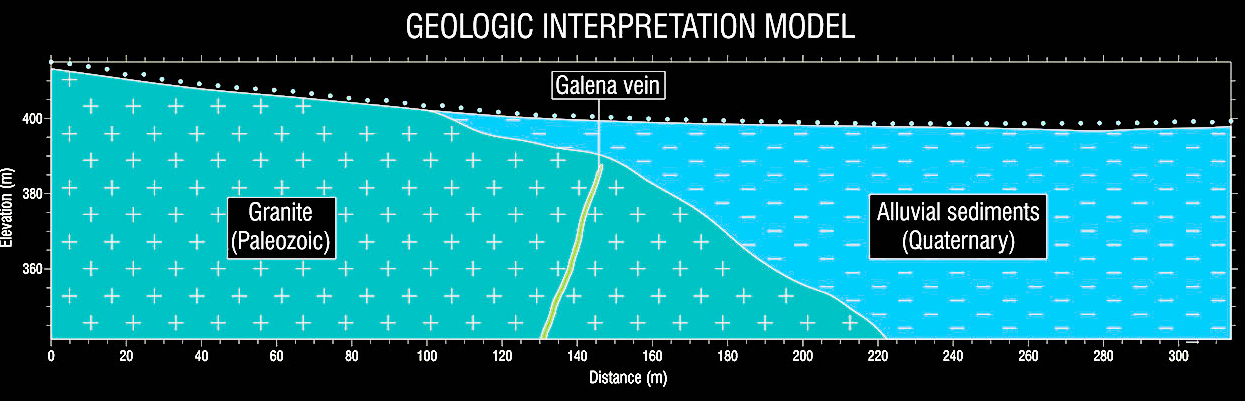
\includegraphics[width=0.8\linewidth]{Figures/InducedPolarization/resistivity-and-chargeability_subsurface_EverestGeophysics.png}

  \tiny[Source: Everest Geophysics (Spain)]
\end{frame}


\begin{frame}{Examples}
  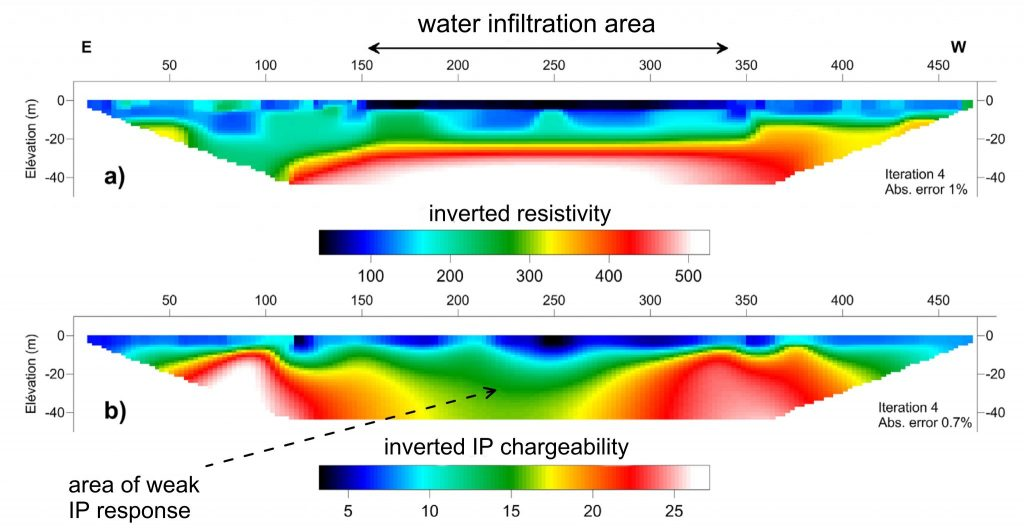
\includegraphics[width=0.8\linewidth]{Figures/InducedPolarization/IP_Guidal.jpg}
\tiny [CITREX At Guidel site (France) the high chargeability is linked with pyrite preserved in non-weathered granites. In the central zone, pyrite has been oxidized and the chargeability is lower.]
\end{frame}


\begin{frame}
  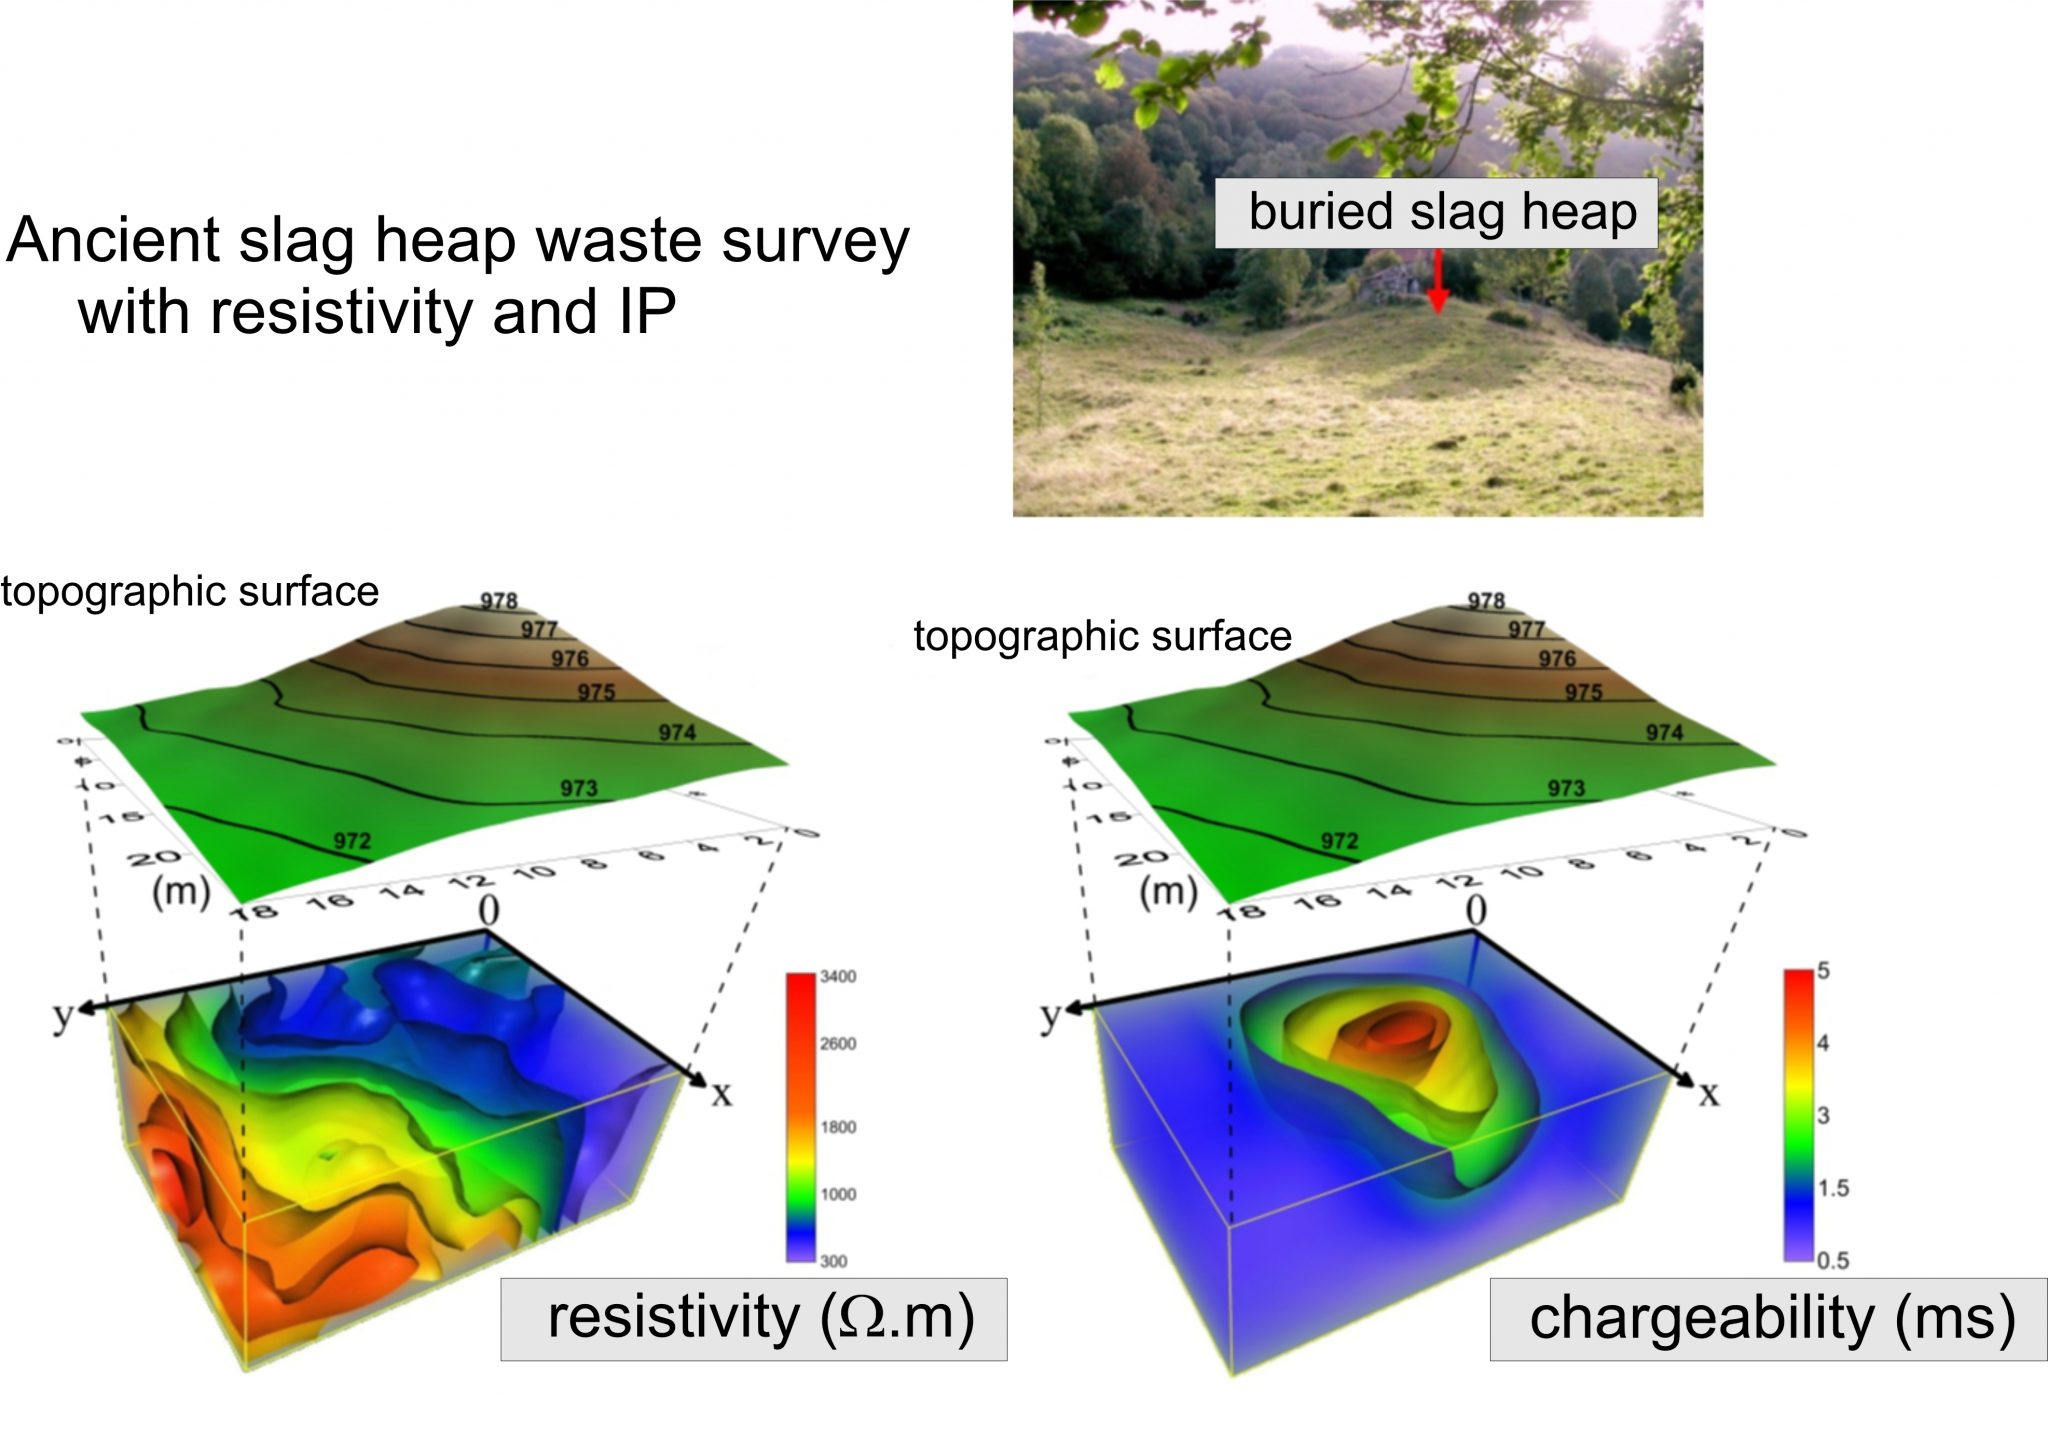
\includegraphics[width=0.8\linewidth]{Figures/InducedPolarization/IPSlagHeap.jpg}
  % Slag heap is Schlackenhalde als abfall von Mine.
  \tiny [ CITREX: On the mining site of Aulus-les-Bains (Ariège, France), IP permits to map an ancient slag heap, where magnetite particles are responsible of the IP signal. One observes that IP and resistivity are fairly independent.]
\end{frame}

\begin{frame}{Examples}
   Share talk from C. Moser at EGU 2022
\end{frame}

\begin{frame}
  \begin{PointSix}{Learning Goals}
    \begin{itemize}
      \item \alert{Polarization.}
      \item \alert{Polarization in the subsurface.}
      \item \alert{Principles of an RC circuit.}
      \item \alert{Definition of chargeability.}
    \end{itemize}
  \end{PointSix}
\end{frame}

\begin{frame}
  \begin{PointSix}{Primer Spectral induced polarization}
       \small 
      The idea of spectral induced polarization is to apply a time variable potential / input current:
      $$
        V(t) = V_0e^{i\omega t}
      $$

      (Clarify complex notation if this is unclear.)
  \end{PointSix}
\end{frame}

\begin{frame}
\begin{eqnarray*}
  V(t) - V_R(t) - V_C(t) = 0 \\
  V_C(t) = \frac{q(t)}{C} \\ 
  V_R(t) = RI \\
  I(t) = \frac{dq}{dt}
 \end{eqnarray*}
\end{frame}

\begin{frame}{Primer Spectral Induced Polarization}
  \begin{eqnarray}
    &V(t) = V_0e^{i\omega t} \\
    &V_c = \frac{q}{C} \\
    &\frac{d}{dt}V_C = I_C \frac{1}{C} \\
    &\rightarrow \underbrace{\frac{1}{i\omega C}}_{Impedance} I_C =  V(t)
  \end{eqnarray}
\end{frame}



\begin{frame}{Primer Spectral Induced Polarization}
  \begin{eqnarray}
    V(t) = I(t)R + \frac{C}{j\omega}I(t) \\
         = (R + \frac{1}{iC\omega})I(t) \\
         = \underbrace{(R - i\frac{1}{C\omega})}_{\text{I(t) and V(t) are phase shifted.}}I(t)
  \end{eqnarray}
\end{frame}